\documentclass[11pt,twoside,a4paper]{article}
\usepackage[utf8]{inputenc}
\usepackage[english,german]{babel}
\usepackage[margin=1in,outer=0.6in,inner=1.4in]{geometry}
%\usepackage[parfill]{parskip} % paragraph indent: uncomment if no paragaph indent is needed
\usepackage{makeidx}
\usepackage[onehalfspacing]{setspace}
\usepackage{fancyhdr}
\usepackage{lastpage}
\usepackage{hyperref}
\usepackage{multicol}
\usepackage{footnote}


\usepackage{graphicx}
\renewcommand{\sffamily}{phv}
\renewcommand{\familydefault}{\sffamily}
\newcommand{\titleText}{Terminalserver}
\newcommand{\authorText}{Luka Kramer, Patrick Günthard}
\newcommand{\dateText}{\today}

\title{\textbf{\titleText}}
\author{\authorText}
\date{\dateText}


\pagestyle{fancy}
\fancyhf{}

\fancyhead[EL]{\titleText}
\fancyhead[OR]{\authorText}
\cfoot{\thepage \space von \pageref{LastPage}}

\begin{document}
	\maketitle
	\tableofcontents
\clearpage
	\section{Wozu dient's?}
        \begin{multicols}{2}
          Terminalserver dienen dazu z.B. Anwendungen auf einem zentralen Server laufen zu lassen auf welche Clients über das Netzwerk zugreifen können. Auch wird diese es für Fernwartung eingesetzt. 
	\end{multicols}
	\section{Wie entstand's?}
	\begin{multicols}{2}
          Das Konzept wurde ursprünglich für die Grossrechner der 1970er und 1980er Jahre. Da es zu teuer gewesen wäre, jedem Arbeitsplatz einen eigener Rechner zur Verfügung zu stellen, wurden sogenannte Thin-Clients installiert welche sich auf den Server einloggten. Zu dieser Zeit waren die Clients direkt über eine RS-232 Schnittstelle mit dem Host verbunden. Heutzutage (2016) werden diese Verbindungen über ein Netzwerk aufgebaut (meist über tcp/ip). 

          Heuzutage haben Terminalserver auch ein neues anwendungsgebiet. Sie werden zur Fernwartung eingesetzt da Clients mitlerweile genug Leistung haben um ein eigenes System auszuführen. 
	\end{multicols}
          \begin{figure}{H}
            \centering
            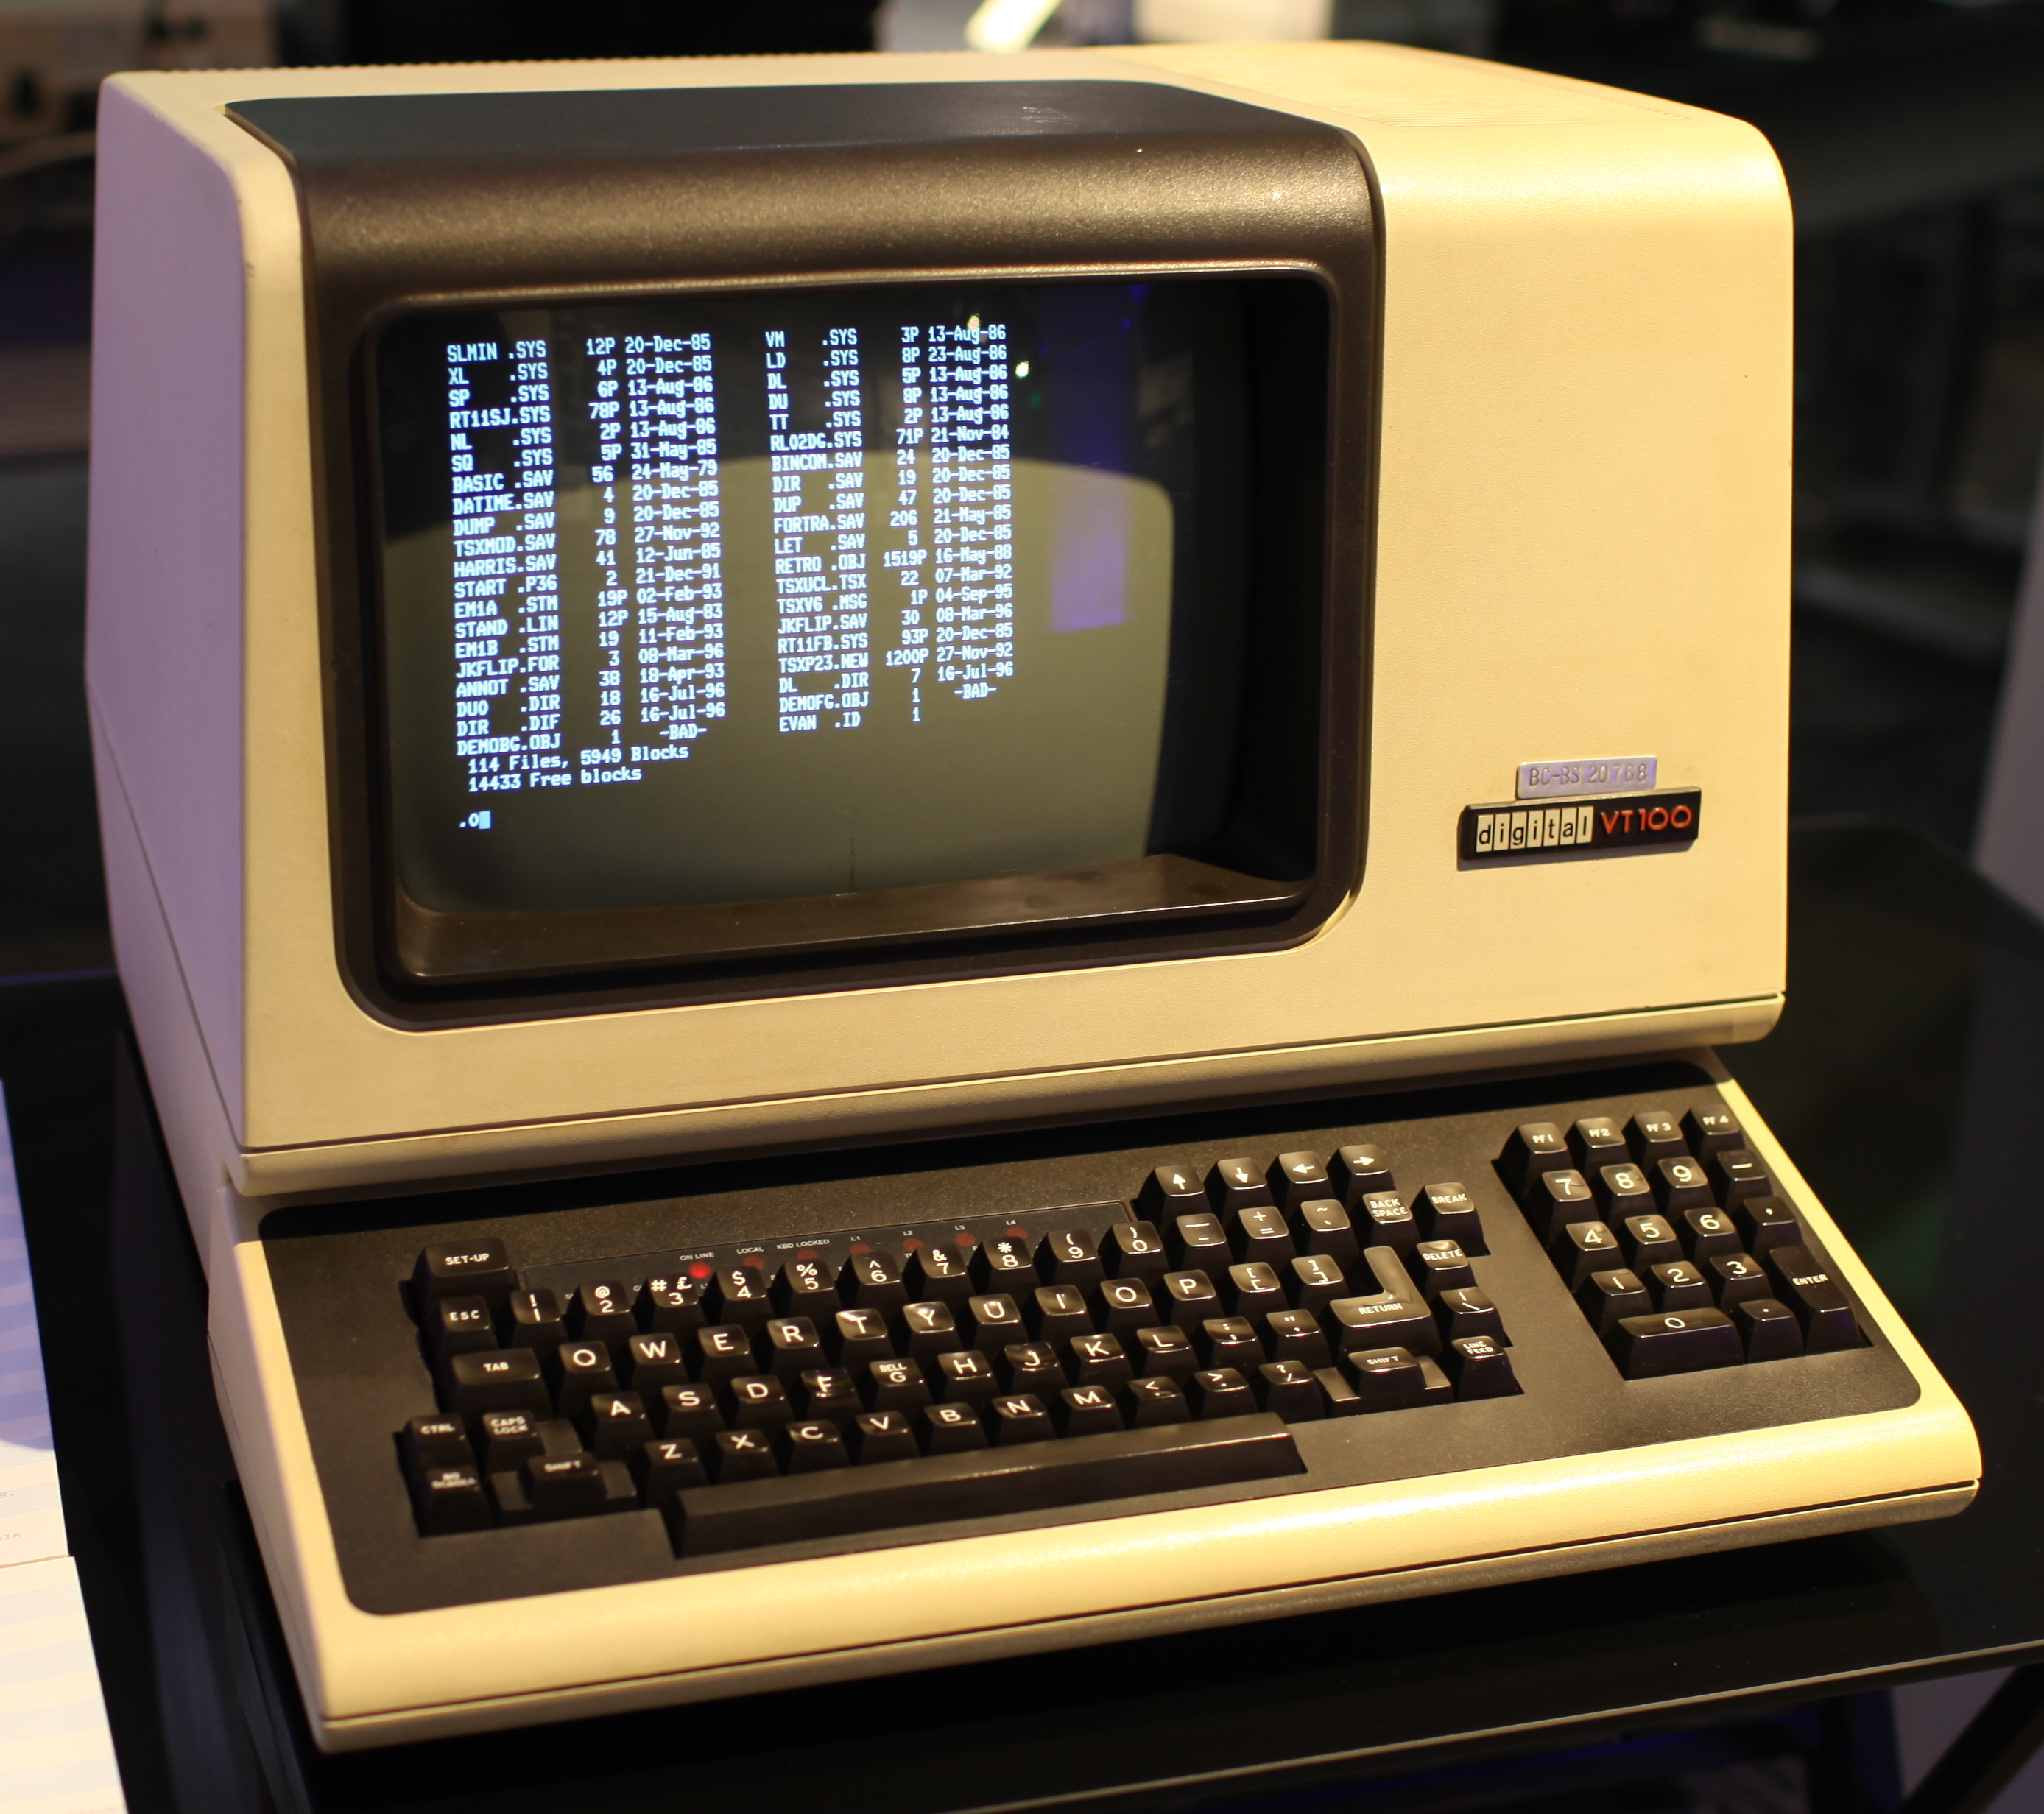
\includegraphics[width=5cm]{terminal}
            \caption{figure}{VT100 Terminal}
          \end{figure}

	\section{Wie funktioniert's?}
	\begin{multicols}{2}
          Auf einem zentralen Server läuft ein Server auf welchen ein Client sich verbindet und einloggt. Beim Loggin wird auf einem Account eingeloggt welcher \textit{auf dem Server} läuft wobei es keine Rolle spielt ob der User-Account lokal oder auf einem LDAP System gespeichert ist. 
	\end{multicols}
        
	\section{Lösungen}
	\begin{multicols}{2}
          \subsection{telnet}
          Telnet ist ein Protokoll für die (unverschlüsselte) Übertragung von Text-basierten Daten. Telnet ist auf fast allen Netzwerkfähigen Systemen verfügbar, auch auf solchen welche auf Windows NT basieren\footnote{\url{http://windows.microsoft.com/en-us/windows/telnet-faq\#1TC=windows-7}}.
          \subsection{SSH}
          \textit{Secure Shell} ist ein Protokoll welches eine verschlüsselte Übertragung zulässt. Es wird hauptsächlich auf UNIX und UNIX-artigen Systemen eingesetzt, es gibt aber auch ports auf die win32 Architektur von Microsoft (2015 wurde von Microsoft angekündigt, SSH auch nativ zu unterstützen \footnote{\url{https://en.wikipedia.org/wiki/Secure_Shell\#cite_note-3}}). Mit SSH lassen sich verschiedene Protokolle übertragen wobei auch auf dem Server laufende X11 GUIs auf dem client angezeigt werden können.
          
	\end{multicols}

	\begin{thebibliography}{9}
        \bibitem[Secure Shell - Wikipedia]{ssh}\url{https://en.wikipedia.org/wiki/Secure_Shell}
        \end{thebibliography}

	
\end{document}